\bibliography{dissertation}
\appendix

\chapter{Appendix A: AI Usage}
\label{appx:ai_prompt}

I did not directly prompt any Large Language Models, or any other AI model, to assist with the writing of my dissertation or implementation. However, as listed in the Supporting Technologies list, I used GitHub Copilot to help with writing some tests for the parser and type checker. I used it via the VS Code extension, which uses the context of your file, to provide advanced AI autocompletion.

% =============================================================================

\chapter{Appendix B: Tokens for Lexical Analysis}
\label{appx:tokens}
Below is the code for how tokens outputted by lexical analysis are defined. 
\begin{lstlisting}
enum TokenType {
    EOF,
    Newline,

    Id,
    UppercaseId,

    If,
    Then,
    Else,

    Match,
    LBrace,
    RBrace,

    IntLit,
    FloatLit,
    StringLit,
    CharLit,
    BoolLit,

    DoubleColon,
    RArrow,
    Forall,
    KWType,
    KWData,

    LParen,
    RParen,

    Lambda,

    Dollar,
    Dot,
    Comma,
    Bar,

    Assignment,
}

struct Token {
    tt: TokenType,
    value: String,
}
\end{lstlisting}

\chapter{Appendix C: How the System Looked During Various Testing Stages}
\section{Testathon}

\begin{figure}[h]
    \centering
    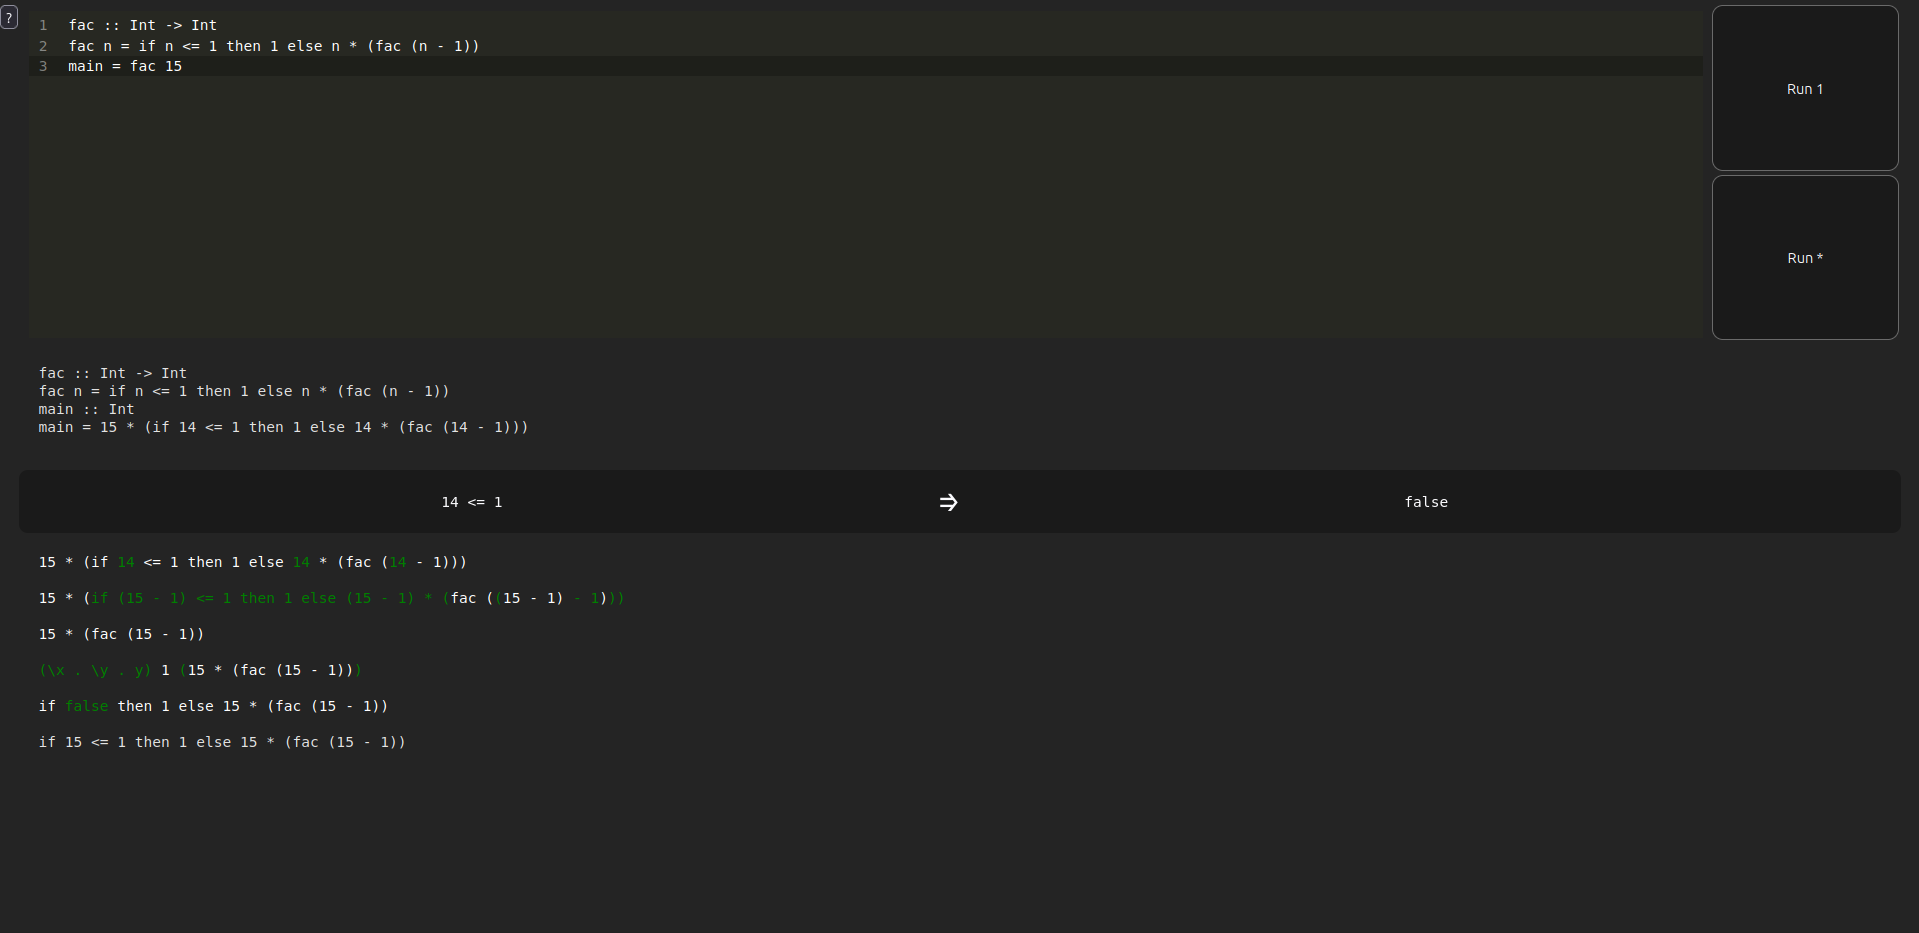
\includegraphics[width=1\linewidth]{images/product_at_testathon.png}
    \caption{The UI as tested in the testathon}
    \label{fig:screenshot_testathon}
\end{figure}

\begin{figure}
    \centering
    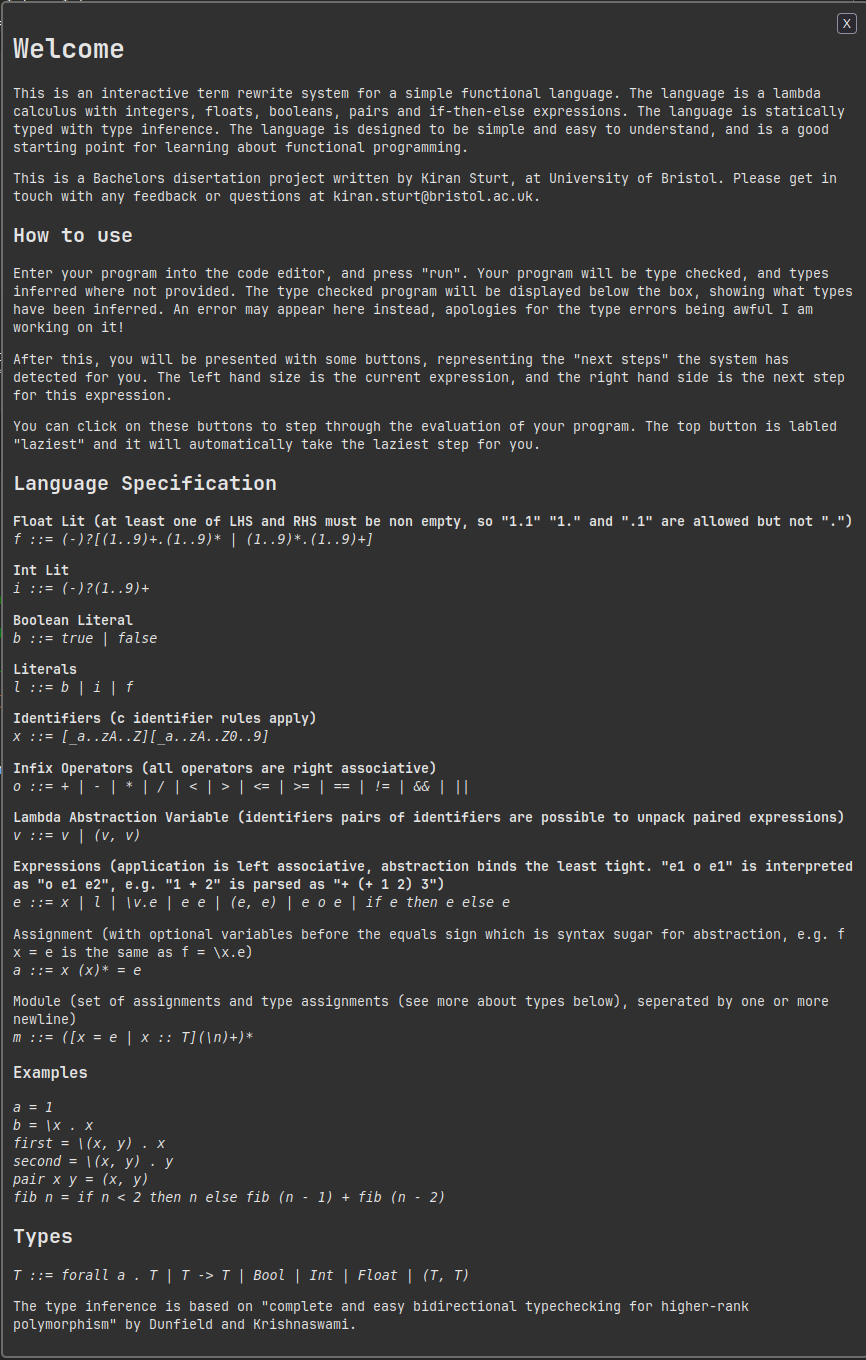
\includegraphics[width=0.9\linewidth]{images/testathon_help_menu.png}
    \caption{The "Help menu" in the testathon. This was spawned by pressing the "?" button in the top left of the UI, and dismissed by pressing the "X" button, or clicking outside of the box}
    \label{fig:screenshot_testathon_2}
\end{figure}